\documentclass[aspectratio=169,11pt,t]{beamer}
% ============================================================
%  ksa-cs-v2: ksa-cs-lecture-template.tex 스타일 + 한글, v2 덱(16:9)용.
%    - 짙은 네이비 헤드라인 (섹션 이름 + 프레임마다 점)
%    - 꽉 찬 파란 제목 막대, 둥근 그림자 블록
%    - 한글: Noto Sans CJK KR (fontspec)
%  사용:
%    \documentclass[aspectratio=169,11pt,t]{beamer}
%    \input{<..>/theme/ksa-cs-v2.tex}
%  ksa-theme.tex 의 매크로(\kb \kq, ksablue/ksared 등)도 같은 이름으로 둔다
%  -> v2 덱 본문을 거의 그대로 옮길 수 있다.
% ============================================================

\usepackage{fontspec}
\usepackage{amsmath,amssymb}
\usepackage{tikz}
\usepackage{listings}
\usepackage{graphicx}
\usepackage{booktabs}
\usepackage{varwidth}
% enumitem 은 넣지 않는다 (beamer 글머리표가 사라진다)

\defaultfontfeatures{Ligatures=TeX}
\setmainfont{Noto Sans CJK KR}
\setsansfont{Noto Sans CJK KR}
\setmonofont{Noto Sans Mono CJK KR}[Scale=0.92]
\usefonttheme{professionalfonts}

% ---------- 기본 틀 ----------
\usetheme{default}
\useinnertheme[shadow=true]{rounded}
\setbeamertemplate{navigation symbols}{}
\setbeamersize{text margin left=1em,text margin right=1em}

% ---------- 색 (템플릿 원본 값) ----------
\definecolor{navydark}{HTML}{191959}
\definecolor{navydim}{HTML}{8888B0}
\definecolor{navytitle}{HTML}{262686}
\definecolor{navyblue}{HTML}{3333B2}
\definecolor{blockbodybg}{HTML}{E9E9F3}
\definecolor{examplegreen}{HTML}{006000}
\definecolor{examplebg}{HTML}{E5EFE5}
\definecolor{alertred}{HTML}{BF0000}
\definecolor{alertbg}{HTML}{F9E5E5}
% ksa-theme.tex 와 같은 이름 (본문 호환)
\colorlet{ksablue}{navytitle}
\colorlet{ksabluedk}{navydark}
\definecolor{ksagold}{HTML}{D6CBB1}
\definecolor{ksagolddk}{HTML}{A9976B}
\colorlet{ksared}{alertred}
\definecolor{ksagray}{HTML}{5B5B5B}

\setbeamercolor{structure}{fg=navyblue}
\setbeamercolor{alerted text}{fg=alertred}
\setbeamercolor{frametitle}{bg=navytitle,fg=white}
\setbeamercolor{title}{fg=white,bg=navytitle}
\setbeamercolor{block title}{bg=navytitle,fg=white}
\setbeamercolor{block body}{bg=blockbodybg,fg=black}
\setbeamercolor{block title example}{bg=examplegreen,fg=white}
\setbeamercolor{block body example}{bg=examplebg,fg=black}
\setbeamercolor{block title alerted}{bg=alertred,fg=white}
\setbeamercolor{block body alerted}{bg=alertbg,fg=black}
\setbeamercolor{item}{fg=navyblue}
\setbeamertemplate{itemize item}[circle]
\setbeamertemplate{itemize subitem}[triangle]

% ---------- 헤드라인: miniframes (섹션 이름 + 점) ----------
\useoutertheme[subsection=false]{miniframes}
\setbeamerfont{section in head/foot}{size=\tiny}
\setbeamercolor{section in head/foot}{bg=navydark,fg=white}
\setbeamercolor{mini frame}{fg=white}
\setbeamertemplate{mini frames}[circle]

% ---------- 제목 막대: 폭 꽉 채움, 두 줄까지 ----------
\setbeamerfont{frametitle}{size=\normalsize,series=\bfseries}
\setbeamertemplate{frametitle}{%
  \nointerlineskip
  \begin{beamercolorbox}[wd=\paperwidth,ht=2.7ex,dp=1.1ex,leftskip=.3cm,rightskip=.3cm]{frametitle}%
    \usebeamerfont{frametitle}\insertframetitle
  \end{beamercolorbox}}

% ---------- 쪽 번호: 오른쪽 아래 ----------
\setbeamertemplate{footline}{%
  \hfill
  {\color{navydim}\scriptsize\insertframenumber\,/\,\inserttotalframenumber}%
  \hspace{3mm}\vspace{2mm}%
}

% ---------- 표지: 템플릿처럼 헤드라인은 그대로, 가운데 둥근 그림자 상자에 제목 한 줄 ----------
% 덱에서:  {\setbeamertemplate{footline}{}\begin{frame}[c,noframenumbering]\titlepage\end{frame}}
\setbeamercolor{title}{fg=white,bg=navyblue}
\makeatletter
\setbeamertemplate{title page}{%
  \vfill
  \centering
  \begin{minipage}{0.84\paperwidth}
  \begin{beamercolorbox}[wd=\linewidth,sep=7pt,center,rounded=true,shadow=true]{title}
    {\usebeamerfont{title}\inserttitle\par}%
    \ifx\insertsubtitle\@empty\else\vskip0.4em{\usebeamerfont{subtitle}\insertsubtitle\par}\fi
  \end{beamercolorbox}
  \end{minipage}\par\vskip1.6em
  {\usebeamerfont{author}\color{navytitle}\insertauthor\par}\vskip0.3em
  {\usebeamerfont{institute}\color{ksagray}\insertinstitute\par}
  \vfill
}
\makeatother
\setbeamerfont{title}{series=\bfseries,size=\Large}
\setbeamerfont{subtitle}{size=\normalsize}
\setbeamerfont{author}{size=\normalsize}
\setbeamerfont{institute}{size=\small}

% ksa-theme 호환: 덱이 \renewcommand{\ksacredit}{..} 를 해도 되게 (꼬리말에는 안 쓴다)
\newcommand{\ksacredit}{}

% ---------- 강조 ----------
\newcommand{\hl}[1]{\textcolor{alertred}{#1}}
\newcommand{\hlb}[1]{\textcolor{navyblue}{#1}}
\newcommand{\kb}[1]{\textbf{\color{ksablue}#1}}
\newcommand{\kq}[1]{\textbf{\color{ksared}#1}}

% ---------- 파이썬 코드 (템플릿과 같은 색) ----------
\definecolor{codekw}{HTML}{0033B3}
\definecolor{codebuiltin}{HTML}{BF0000}
\definecolor{codestr}{HTML}{067D17}
\definecolor{codecomment}{HTML}{8C8C8C}
\definecolor{codenum}{HTML}{1750EB}
\lstdefinestyle{py}{
  language=Python, basicstyle=\ttfamily\scriptsize,
  keywordstyle=\color{codekw}\bfseries, stringstyle=\color{codestr},
  commentstyle=\color{codecomment}\itshape, numberstyle=\color{codenum},
  emph={print,len,range,sum,input,int,str,float,list,dict,append,remove,sorted,abs,min,max},
  emphstyle=\color{codebuiltin}, showstringspaces=false, keepspaces=true,
  columns=fixed, basewidth=0.52em, aboveskip=1mm, belowskip=1mm, xleftmargin=2mm,
  breaklines=true
}
\lstset{style=py}

% 원본 덱 (ksa-theme): slides/v2/ml1/week02/linear_regression/ -- 그림은 거기 figs/ 를 그대로 쓴다
\setbeamerfont{author}{size=\normalsize}
\setbeamerfont{institute}{size=\small}
\graphicspath{{../../../v2/ml1/week02/linear_regression/figs/}{../../../assets/}}
\makeatletter
\newcommand{\markpage}[1]{\protected@write\@auxout{}{\string\newlabel{#1}{{\the\c@framenumber}{}}}\hypertarget{#1}{}}
\newcommand{\pref}[1]{\hyperlink{#1}{\textcolor{ksagolddk}{(p.\ref{#1})}}}
\makeatother

\renewcommand{\ksacredit}{Machine Learning and Deep Learning \,\textperiodcentered\, 선형회귀}
\title{선형회귀 (Linear Regression)}
\subtitle{직선 하나로 예측하기, 그리고 곡선까지}
\author{Machine Learning and Deep Learning}
\institute{한국과학영재학교 (KSA)}
\date{}
\begin{document}
{\setbeamertemplate{footline}{}\begin{frame}[c,noframenumbering]\titlepage\end{frame}}

\section{질문}
% --- 오늘의 질문
\begin{frame}{오늘의 질문}
\vfill
\centering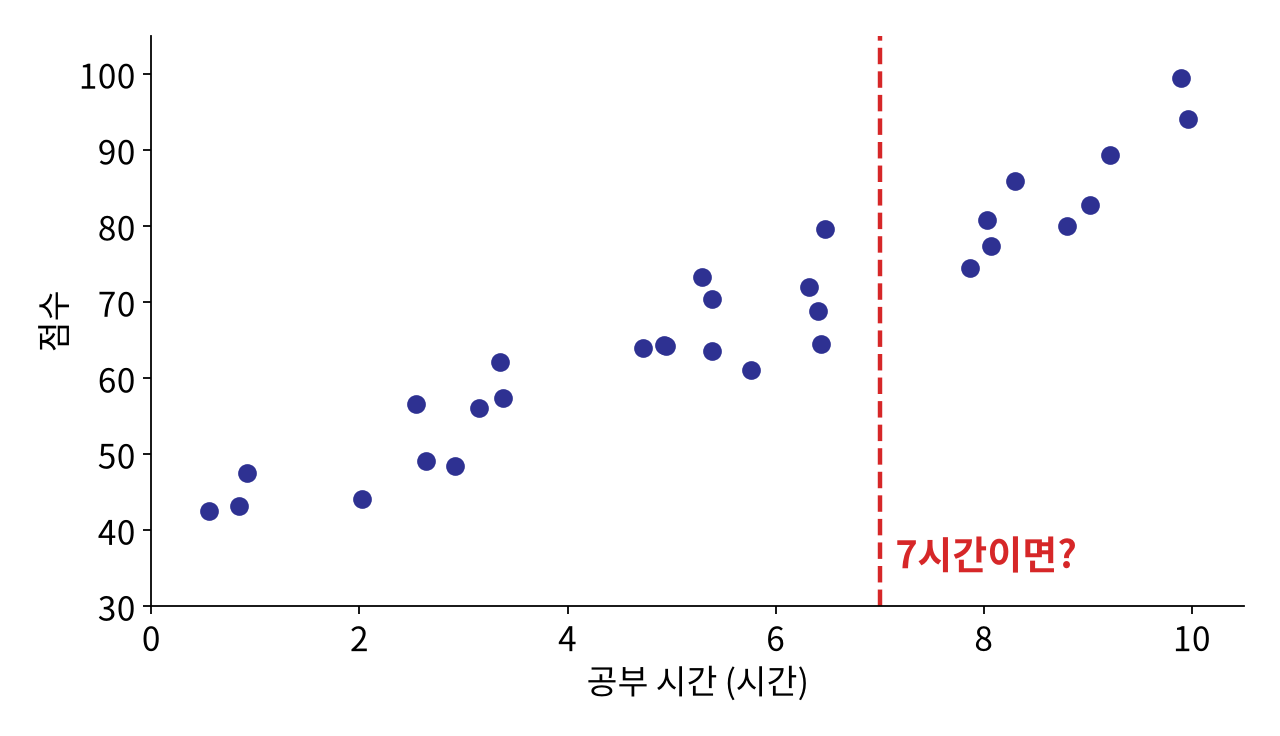
\includegraphics[width=0.62\linewidth]{lr_hook.png}\par\vskip0.3em
{\large 학생 30명의 공부 시간과 점수. \kq{7시간 공부하면 몇 점일까?}}
\vfill
\note{학생 30명의 공부 시간과 시험 점수입니다. 공부를 많이 할수록 점수가 높은 경향이 보입니다. 그러면 7시간 공부한 학생은 몇 점쯤 받을까요? 이렇게 숫자를 예측하는 문제를 회귀라고 하고, 오늘은 가장 기본적인 방법인 선형회귀를 배웁니다.}
\end{frame}

\section{비용}
% --- 모델
\begin{frame}{직선을 긋는다}
\vfill
\centering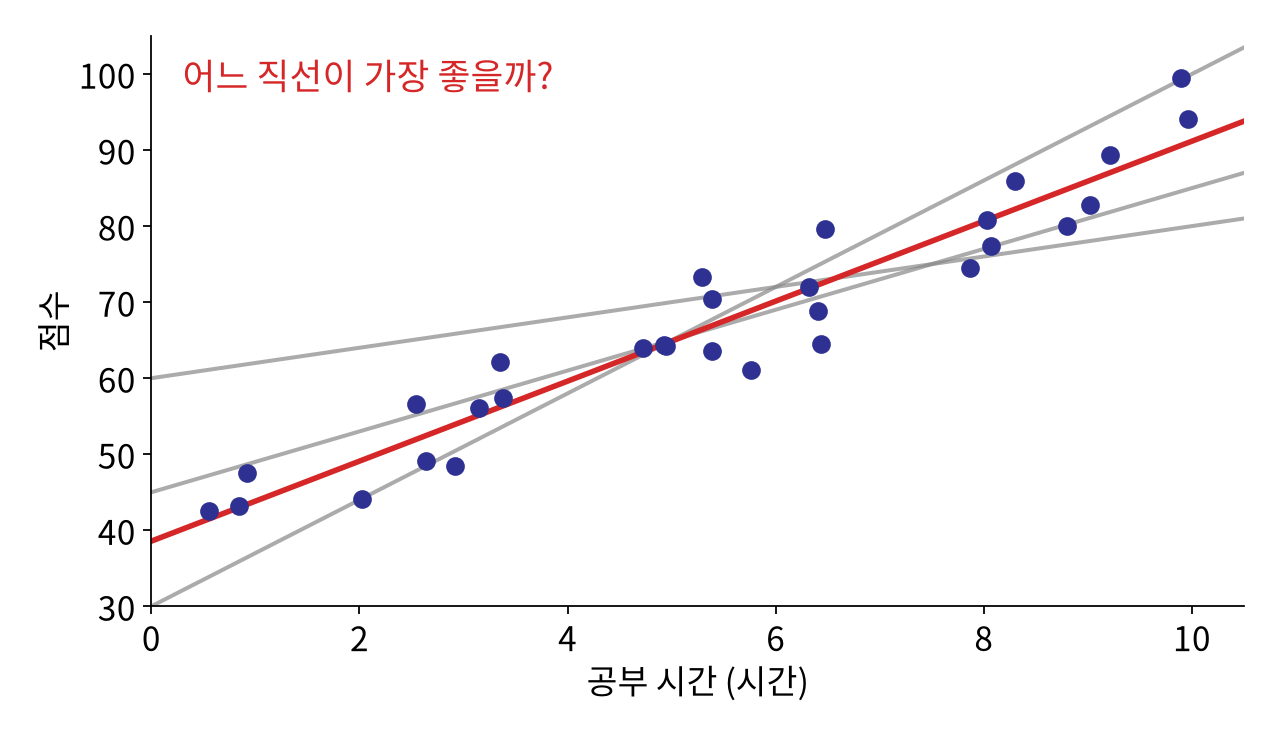
\includegraphics[width=0.47\linewidth]{lr_lines.png}\par\vskip0.3em
{\LARGE\[ h_{\boldsymbol w}(x) = w_0 + w_1 x \]}
{\small $w_0$: 절편 \qquad $w_1$: 기울기 (1시간 더 하면 몇 점 오르나)}
\vfill
\note{점들 사이로 직선을 하나 그어서, 그 직선으로 예측합니다. 직선은 절편 w0와 기울기 w1, 숫자 두 개로 정해집니다. w1은 공부를 1시간 더 하면 점수가 몇 점 오르는지를 뜻합니다. 그런데 그을 수 있는 직선은 무수히 많습니다. 어느 직선이 가장 좋은지 기준이 필요합니다.}
\end{frame}

% --- 비용
\begin{frame}{오차를 제곱해서 평균: 비용 $J$}
\markpage{cost}
\vfill
\begin{columns}[c]
\begin{column}{0.52\textwidth}\centering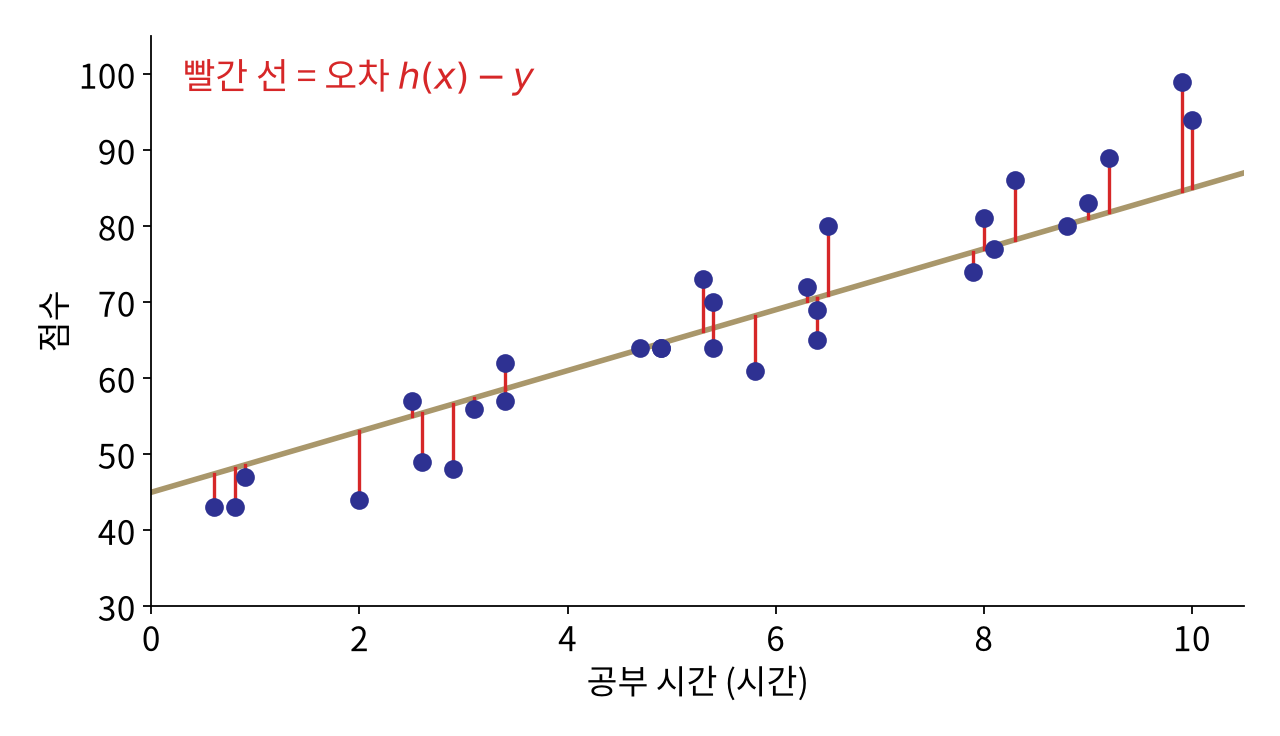
\includegraphics[width=\linewidth]{lr_residuals.png}\end{column}
\begin{column}{0.44\textwidth}
{\large\[ J(\boldsymbol w) = \frac{1}{2m}\sum_{i=1}^{m}\big(h_{\boldsymbol w}(x^{(i)}) - y^{(i)}\big)^2 \]}\vskip0.4em
{\small $m$: 데이터 수 (30명) \quad 빨간 선: 오차}\\[0.5em]
{\small 제곱: 음수 오차와 양수 오차가 상쇄되지 않게}\\[0.2em]
{\small $\frac12$: 미분할 때 2와 약분되라고 붙인 것}
\end{column}
\end{columns}
\vfill
\note{기준은 오차입니다. 각 학생마다 직선이 예측한 점수와 실제 점수의 차이, 빨간 선이 오차입니다. 오차를 그냥 더하면 위아래가 상쇄되니까 제곱해서 더하고, 데이터 수로 나눠 평균을 냅니다. 앞의 2분의 1은 미분할 때 지수 2와 약분되라고 붙인 것입니다. 이 값을 비용 J라고 부르고, J가 가장 작은 직선이 가장 좋은 직선입니다.}
\end{frame}

% --- 그릇
\begin{frame}{$J$ 는 그릇 모양}
\vfill
\centering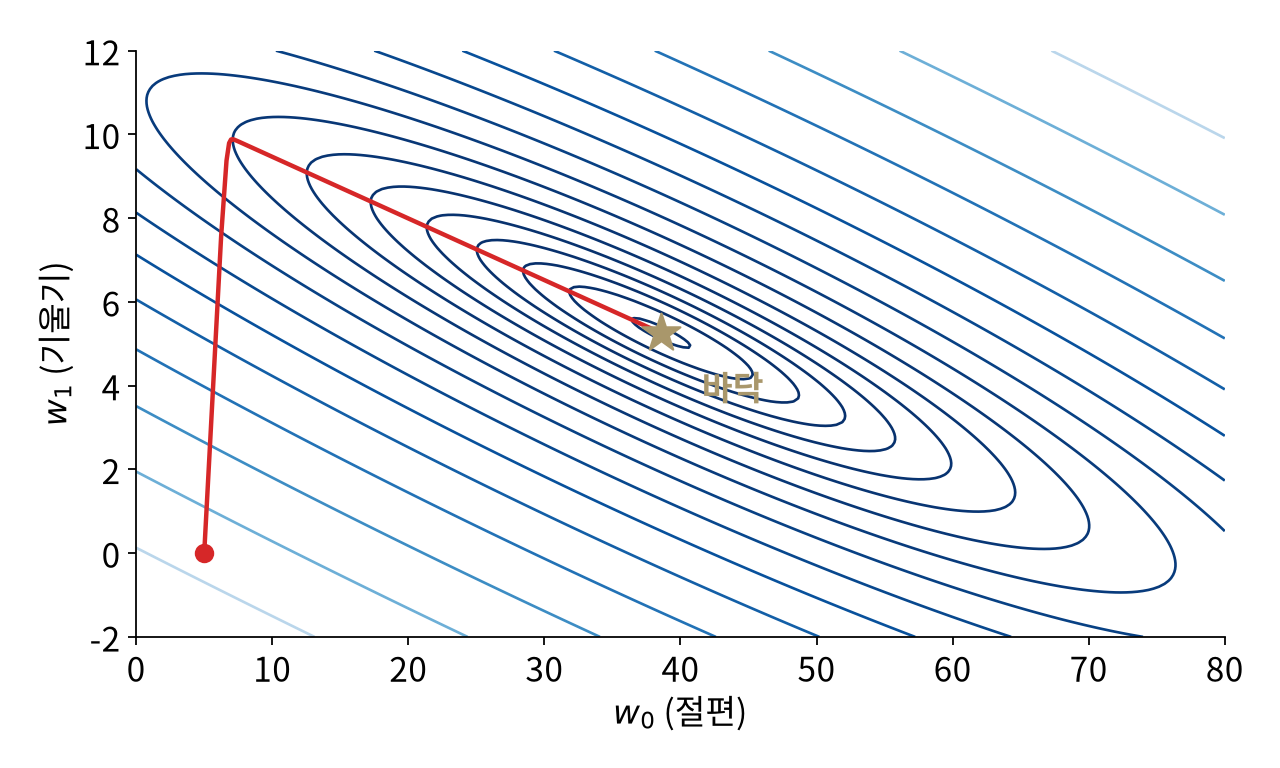
\includegraphics[width=0.56\linewidth]{lr_bowl.png}\par\vskip0.2em
{\small $w_0$, $w_1$ 를 바꿀 때마다 $J$ 가 달라진다. 등고선의 중심 = 가장 좋은 직선. 빨간 선: 경사하강법이 걸어간 길}
\vfill
\note{w0와 w1을 바꿔 가며 J를 계산하면 이렇게 그릇 모양이 됩니다. 등고선 지도로 그렸는데, 가운데 별이 바닥, 즉 J가 가장 작은 곳입니다. 그릇의 바닥은 하나뿐이라서, 어디서 출발하든 내리막을 따라가면 같은 바닥에 도착합니다. 빨간 선이 경사하강법이 실제로 걸어간 길입니다.}
\end{frame}

\section{경사하강법}
% --- 경사하강법
\begin{frame}{경사하강법: 기울기 반대로 한 걸음}
\markpage{gd}
\vfill
\centering
{\Large\[ w_j \;\leftarrow\; w_j - \alpha\,\frac{\partial J}{\partial w_j} \]}\vskip0.4em
{\large\[ \frac{\partial J}{\partial w_0} = \frac{1}{m}\sum_{i=1}^{m}\big(h(x^{(i)}) - y^{(i)}\big) \qquad
\frac{\partial J}{\partial w_1} = \frac{1}{m}\sum_{i=1}^{m}\big(h(x^{(i)}) - y^{(i)}\big)\,x^{(i)} \]}\vskip0.4em
{\small $\alpha$: 학습률 (한 걸음의 크기) \qquad 오차 $\times$ 입력의 평균만큼 고친다}
\vfill
\note{바닥을 찾는 방법이 경사하강법입니다. 지금 위치에서 J가 늘어나는 방향, 즉 기울기를 구해서 그 반대로 학습률 알파만큼 걷습니다. 기울기는 아래 두 식입니다. w0 쪽은 오차의 평균, w1 쪽은 오차 곱하기 입력의 평균입니다. 예측이 크게 틀린 학생일수록, 그리고 공부 시간이 긴 학생일수록 w1을 크게 고칩니다. 실습에서 이 두 줄을 직접 구현합니다.}
\end{frame}

% --- 학습률
\begin{frame}{학습률은 적당히}
\vfill
\centering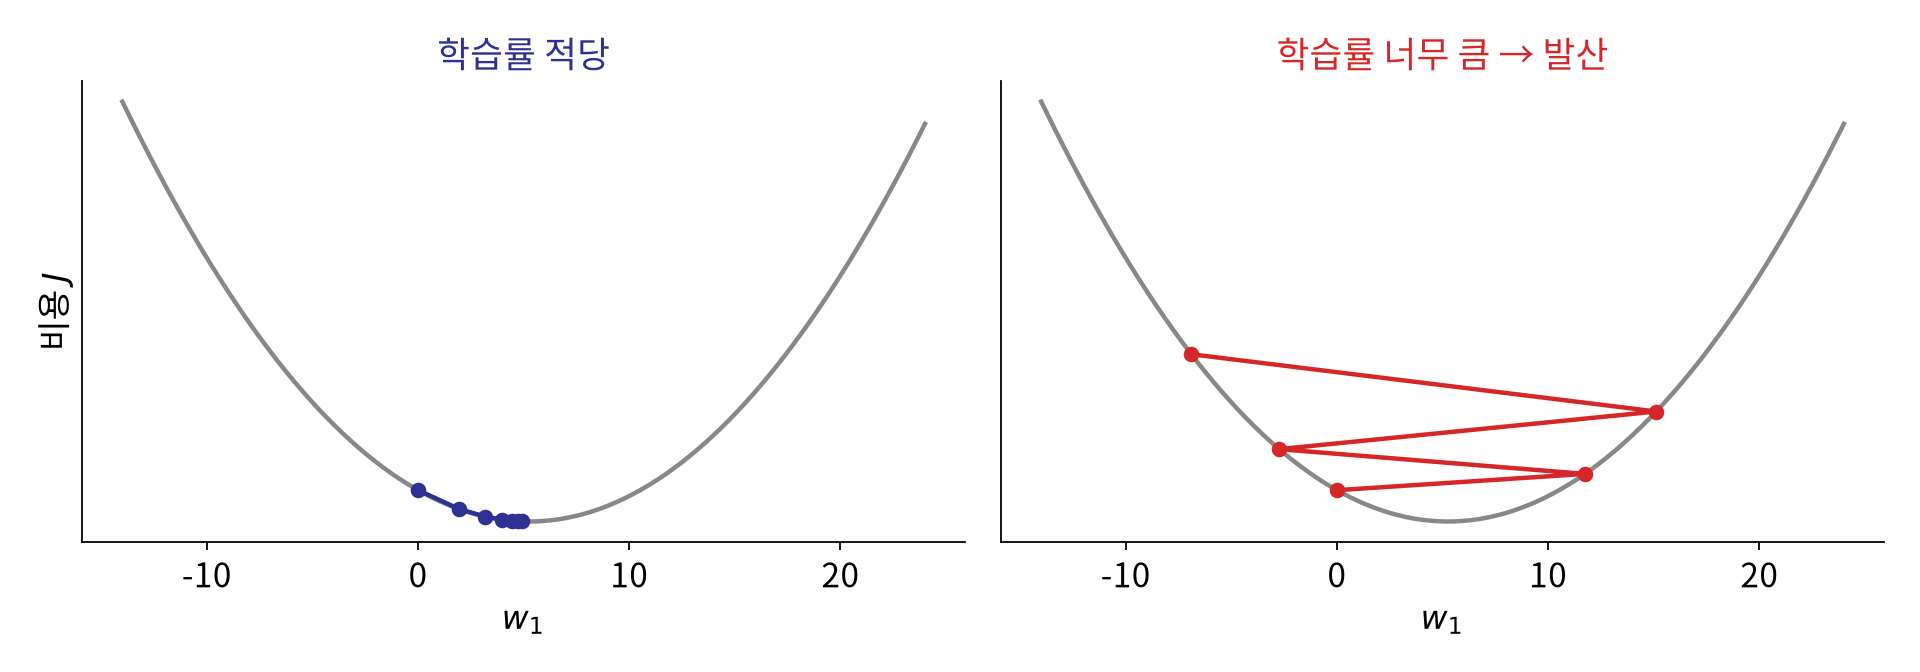
\includegraphics[width=0.86\linewidth]{lr_alpha.png}\par\vskip0.3em
{\large 너무 작으면 느리고, \kq{너무 크면 바닥을 건너뛰며 튕겨 나간다}}
\vfill
\note{학습률이 적당하면 왼쪽처럼 바닥으로 차근차근 내려갑니다. 그런데 너무 크면 오른쪽처럼 바닥을 건너뛰어 반대편으로 가고, 매번 더 높은 곳에 떨어지면서 튕겨 나갑니다. 이걸 발산이라고 합니다. 너무 작으면 바닥까지 한참 걸리고요. 그래서 학습률은 적당히 골라야 합니다.}
\end{frame}

% --- 결과
\begin{frame}{바닥에 도착하면}
\vfill
\centering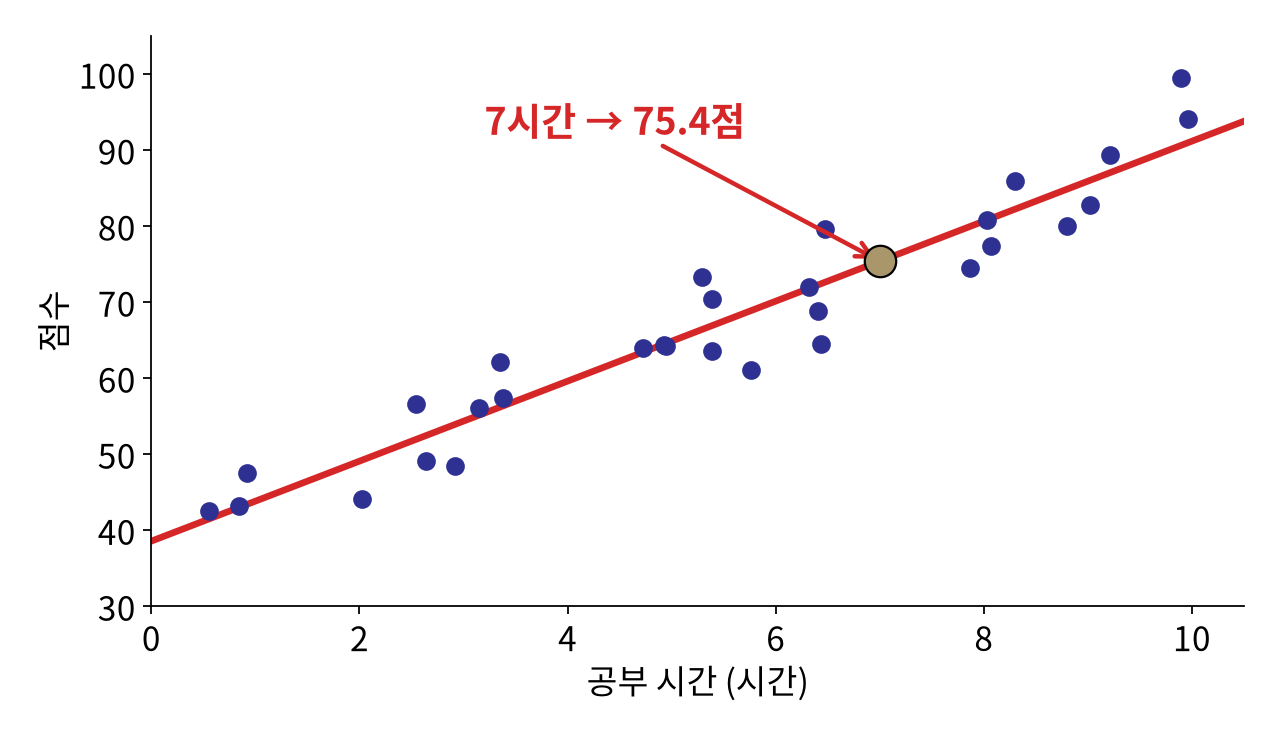
\includegraphics[width=0.6\linewidth]{lr_fit.png}\par\vskip0.3em
{\large $h(x) = 38.6 + 5.25\,x$ \qquad \kq{7시간 $\to$ 75.3점}}
\vfill
\note{바닥에 도착하면 절편 38.6, 기울기 5.25인 직선이 나옵니다. 공부를 1시간 더 할 때마다 약 5점씩 오른다는 뜻입니다. 7을 넣으면 75.3점. 처음 질문의 답입니다.}
\end{frame}

% --- 손으로 풀기: 문제
\begin{frame}{한 문제, 두 가지 풀이}
\vfill
\centering
{\large 점 $(1,2),\ (2,4),\ (3,5)$ 에 직선 $h(x) = w_0 + w_1 x$ 를 맞춘다}\vskip0.8em
\begin{tabular}{c|ccc}
$x$ & 1 & 2 & 3 \\ \hline
$y$ & 2 & 4 & 5
\end{tabular}\vskip0.8em
{\large \kq{$J$ 가 가장 작은 $w_0,\ w_1$ 은?}}\vskip0.6em
{\small 풀이 A: 경사하강법으로 걸어서 \qquad 풀이 B: 식을 풀어서 바로}
\vfill
\note{작은 문제 하나를 두 가지 방법으로 풉니다. 점은 세 개, 1에 2, 2에 4, 3에 5입니다. 직선 h는 w0 더하기 w1 곱하기 x이고, 비용 J가 가장 작은 w0와 w1을 찾습니다. 하나는 방금 배운 경사하강법으로 한 걸음씩 걸어서, 다른 하나는 식을 세워서 바로 풉니다. 같은 답이 나오는지 보세요.}
\end{frame}

% --- 풀이 A
\begin{frame}{풀이 A: 경사하강법 ($\alpha = 0.1$, $w_0 = w_1 = 0$ 에서 출발)}
\vfill
\centering
{\small 첫 걸음: \; 오차 $h - y = -2,\ -4,\ -5$ \quad
$\dfrac{\partial J}{\partial w_0} = \dfrac{-11}{3} \approx -3.67$ \quad
$\dfrac{\partial J}{\partial w_1} = \dfrac{-2 - 8 - 15}{3} \approx -8.33$}\vskip0.3em
{\small $w_0 \leftarrow 0 + 0.1 \times 3.67 = 0.37$ \qquad $w_1 \leftarrow 0 + 0.1 \times 8.33 = 0.83$}\vskip0.8em
\begin{tabular}{r|rrr}
걸음 & $w_0$ & $w_1$ & $J$ \\ \hline
0 & 0 & 0 & 7.50 \\
1 & 0.37 & 0.83 & 1.51 \\
2 & 0.53 & 1.20 & 0.32 \\
3 & 0.60 & 1.37 & 0.09 \\
10 & 0.66 & 1.50 & 0.028 \\
400 & 0.667 & 1.500 & 0.0278
\end{tabular}\vskip0.5em
{\large \kq{수백 걸음 뒤 $w_0 \approx 0.667,\ w_1 \approx 1.5$}}
\vfill
\note{경사하강법으로 풉니다. 학습률은 0.1, 출발점은 w0도 w1도 0입니다. 첫 걸음을 직접 계산해 보면, 예측이 모두 0이라 오차는 마이너스 2, 마이너스 4, 마이너스 5입니다. w0 기울기는 오차의 평균, 마이너스 11 나누기 3, 약 마이너스 3.67. w1 기울기는 오차 곱하기 x의 평균, 마이너스 2, 마이너스 8, 마이너스 15를 더해 3으로 나눈 마이너스 8.33입니다. 기울기 반대로 0.1만큼 가니 w0는 0.37, w1은 0.83이 되고 J는 7.5에서 1.51로 줄었습니다. 같은 계산을 반복하면 표처럼 J가 줄어듭니다. 10걸음에서 이미 거의 다 왔고, 400걸음 뒤에는 w0 0.667, w1 1.5에 도착합니다. 끝까지 가려면 반복이 필요하다는 점을 기억하세요.}
\end{frame}

% --- 풀이 B
\begin{frame}{풀이 B: 기울기를 0 으로 놓고 바로 풀기}
\vfill
\centering
{\small 바닥에서는 기울기가 0 이다: \; $\dfrac{\partial J}{\partial w_0} = 0,\ \ \dfrac{\partial J}{\partial w_1} = 0$}\vskip0.5em
{\large\[ \begin{aligned}
3\,w_0 + 6\,w_1 &= 11 &&\leftarrow\ \textstyle\sum x = 6,\ \sum y = 11 \\
6\,w_0 + 14\,w_1 &= 25 &&\leftarrow\ \textstyle\sum x^2 = 14,\ \sum xy = 25
\end{aligned} \]}\vskip0.3em
{\small 첫 식 $\times 2$ 를 빼면 \; $2\,w_1 = 3$ \; $\Rightarrow$ \; $w_1 = 1.5$, \quad $w_0 = (11 - 9)/3 = 2/3$}\vskip0.8em
{\large\[ \mathbf{w} = (X^\top X)^{-1} X^\top \mathbf{y} \]}\vskip0.2em
{\large \kq{한 번에 $w_0 = 0.667,\ w_1 = 1.5$}}
\vfill
\note{이번에는 걸어가지 않고 바닥의 조건을 바로 씁니다. 바닥에서는 두 기울기가 모두 0입니다. 기울기 식에 0을 놓고 정리하면 식이 두 개 나옵니다. 3 w0 더하기 6 w1은 11, 6 w0 더하기 14 w1은 25입니다. 숫자는 x의 합 6, y의 합 11, x 제곱의 합 14, x 곱하기 y의 합 25에서 나옵니다. 첫 식에 2를 곱해서 빼면 2 w1이 3, 그러니 w1은 1.5이고, w0는 11 빼기 9를 3으로 나눈 3분의 2입니다. 걸음 수 없이 한 번에 나왔습니다. 특징이 많을 때는 이 계산을 행렬로 쓴 정규방정식, w는 X 전치 X의 역행렬 곱하기 X 전치 y입니다.}
\end{frame}

% --- 비교
\begin{frame}{두 풀이는 같은 답, 무엇이 다른가}
\vfill
\centering
\renewcommand{\arraystretch}{1.3}
\begin{tabular}{p{2.4cm}p{5.2cm}p{5.2cm}}
 & \textbf{A. 경사하강법} & \textbf{B. 바로 풀기 (정규방정식)} \\ \hline
답 & $w_0 \approx 0.667,\ w_1 \approx 1.5$ (반복 후) & $w_0 = 2/3,\ w_1 = 3/2$ (정확) \\
준비 & 학습률 $\alpha$, 출발점, 걸음 수 & 없음 \\
비용 & 한 걸음이 싸다, 걸음을 반복 & $d\times d$ 역행렬, 특징 $d$ 개면 약 $d^3$ \\
쓸 수 있는 곳 & 로지스틱회귀, 신경망까지 그대로 & 선형회귀처럼 닫힌 해가 있을 때만
\end{tabular}\vskip0.8em
{\large \kq{특징이 적은 선형회귀는 B, 데이터와 특징이 크거나 다른 모델은 A}}
\vfill
\note{두 풀이는 같은 답을 줍니다. 차이는 방법입니다. 경사하강법은 학습률과 출발점, 걸음 수를 정해야 하고 반복해야 하지만, 한 걸음이 싸서 데이터와 특징이 아주 커도 됩니다. 정규방정식은 준비가 필요 없고 정확한 답을 한 번에 주지만, 특징이 d개면 d 곱하기 d 행렬의 역행렬을 구해야 해서 대략 d의 세제곱만큼 비용이 듭니다. 더 중요한 것은, 닫힌 해가 있는 건 선형회귀 같은 경우뿐이라는 점입니다. 다음 주 로지스틱회귀와 뒤의 신경망에는 이런 식이 없어서 경사하강법으로 풀어야 합니다. 그래서 선형회귀에서 경사하강법을 연습해 두는 것입니다.}
\end{frame}

% --- 평가
\begin{frame}{얼마나 잘 맞나: RMSE와 $R^2$}
\vfill
\centering
{\large
\begin{tabular}{lll}
\textbf{RMSE} & $\sqrt{\tfrac{1}{m}\sum (h - y)^2}$ & \kb{4.36점}: 평균적으로 이만큼 틀린다 (점수와 같은 단위)\\[0.8em]
$\boldsymbol{R^2}$ & $1 - \dfrac{\sum (h-y)^2}{\sum (\bar y - y)^2}$ & \kb{0.916}: 평균으로만 찍을 때보다 오차가 91.6\% 줄었다
\end{tabular}}\vskip1.0em
{\small 평가할 때는 $\frac12$ 없이 그냥 평균 (비용 $J$ 의 $\frac12$ 은 미분 편의용 \pref{cost})}
\vfill
\note{직선이 얼마나 잘 맞는지 숫자로 말하는 방법이 두 가지 있습니다. RMSE는 오차 제곱 평균에 루트를 씌운 것으로, 점수와 같은 단위라서 평균적으로 4.4점쯤 틀린다고 읽으면 됩니다. R 제곱은 모든 학생에게 평균 점수만 찍어 줬을 때와 비교해서 오차가 얼마나 줄었는지입니다. 0.916이면 91.6퍼센트 줄었다는 뜻이고, 1이면 완벽합니다. 평가할 때는 비용 J의 2분의 1을 빼고 계산합니다.}
\end{frame}

\section{곡선}
% --- 곡선
\begin{frame}{데이터가 곡선이면?}
\vfill
\centering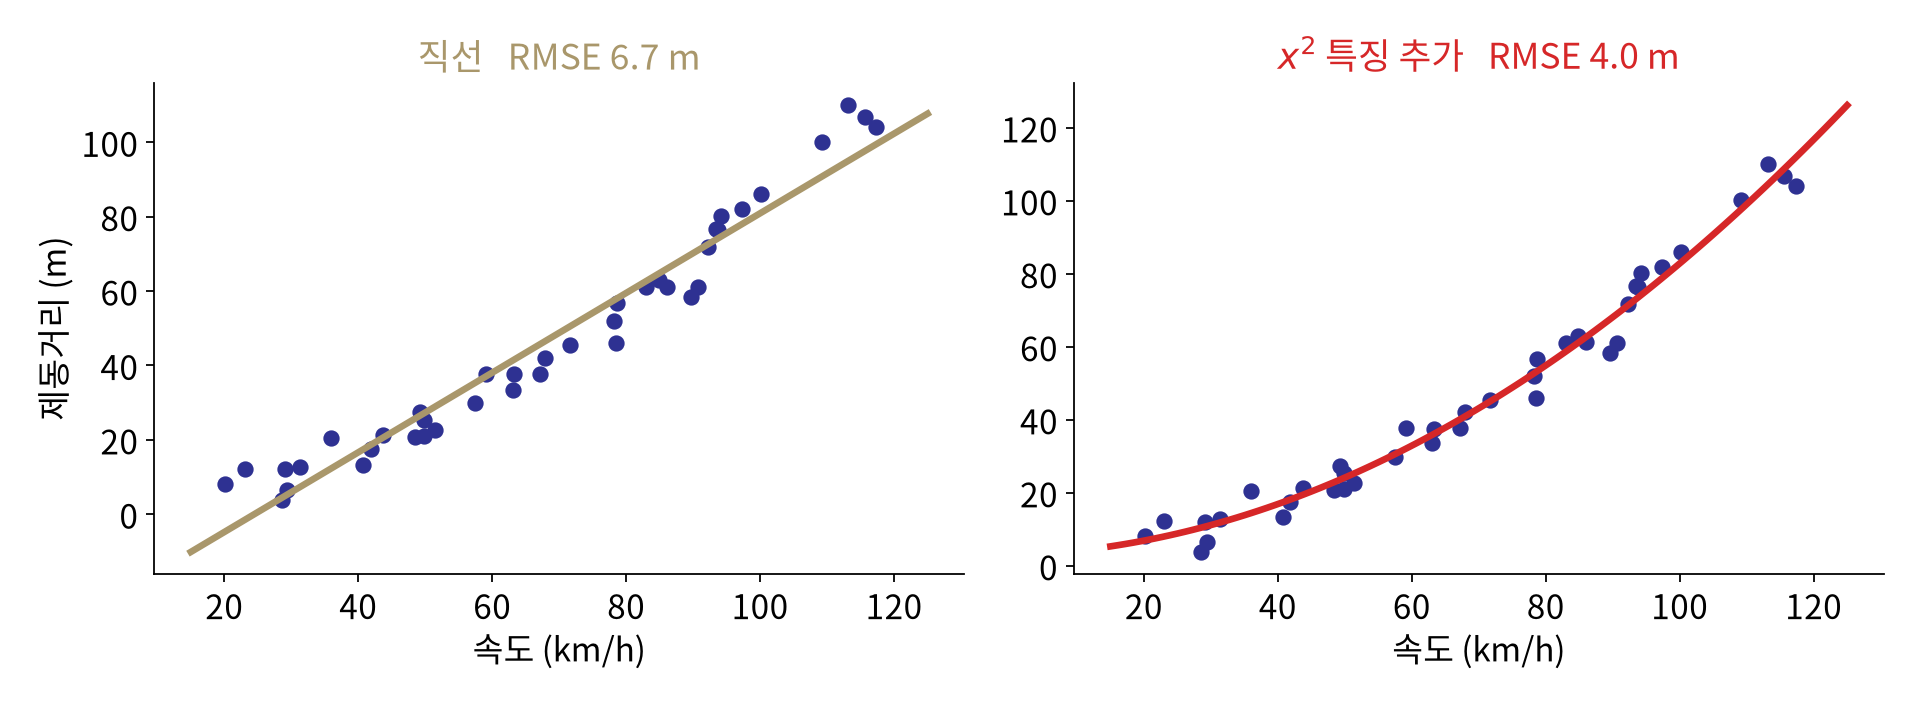
\includegraphics[width=0.9\linewidth]{lr_brake.png}\par\vskip0.3em
{\large 속도 $\to$ 제동거리: $x^2$ 을 \textbf{특징으로 하나 더} 넣으면 \kb{RMSE 6.7 m $\to$ 4.0 m}}
\vfill
\note{이번에는 자동차 속도와 제동거리입니다. 빠를수록 제동거리가 더 가파르게 늘어나는 곡선입니다. 직선으로는 RMSE 6.7미터인데, 속도의 제곱을 특징으로 하나 더 넣어서 h는 w0 더하기 w1 x 더하기 w2 x 제곱으로 바꾸면 4.0미터로 줄어듭니다. 곡선을 그렸는데 이것도 선형회귀입니다. 왜 그럴까요?}
\end{frame}

% --- 선형의 뜻
\begin{frame}{``선형''은 $w$ 에 대해 선형이라는 뜻}
\vfill
\centering
{\Large\[ h(x) = w_0 + w_1\,\underbrace{x}_{\text{feature 1}} + w_2\,\underbrace{x^2}_{\text{feature 2}} \]}\vskip0.6em
{\large $x^2$ 을 새 열로 미리 계산해 두면, $w$ 에 대해서는 여전히 \kb{곱하고 더하기}뿐}\\[0.6em]
{\small 비용 $J$ 도 여전히 그릇 모양 $\to$ 경사하강법 그대로 \pref{gd}}\\[0.8em]
\kq{$h = w_0 + \sin(w_1 x)$ 는? $\to$ $w$ 에 대해 선형이 아니다}
\vfill
\note{선형회귀의 선형은 x에 대해 직선이라는 뜻이 아니라, 가중치 w에 대해 선형이라는 뜻입니다. x 제곱을 미리 계산해서 새 열로 붙여 두면, 모델은 여전히 특징에 w를 곱해서 더하는 것뿐입니다. 그래서 비용 J도 그릇 모양 그대로고, 경사하강법도 그대로 씁니다. 반대로 w가 사인 안에 들어가면 w에 대해 선형이 아니라서 선형회귀가 아닙니다.}
\end{frame}

% --- 로그 변환
\begin{frame}{점점 덜 늘어나면: 로그 변환}
\vfill
\centering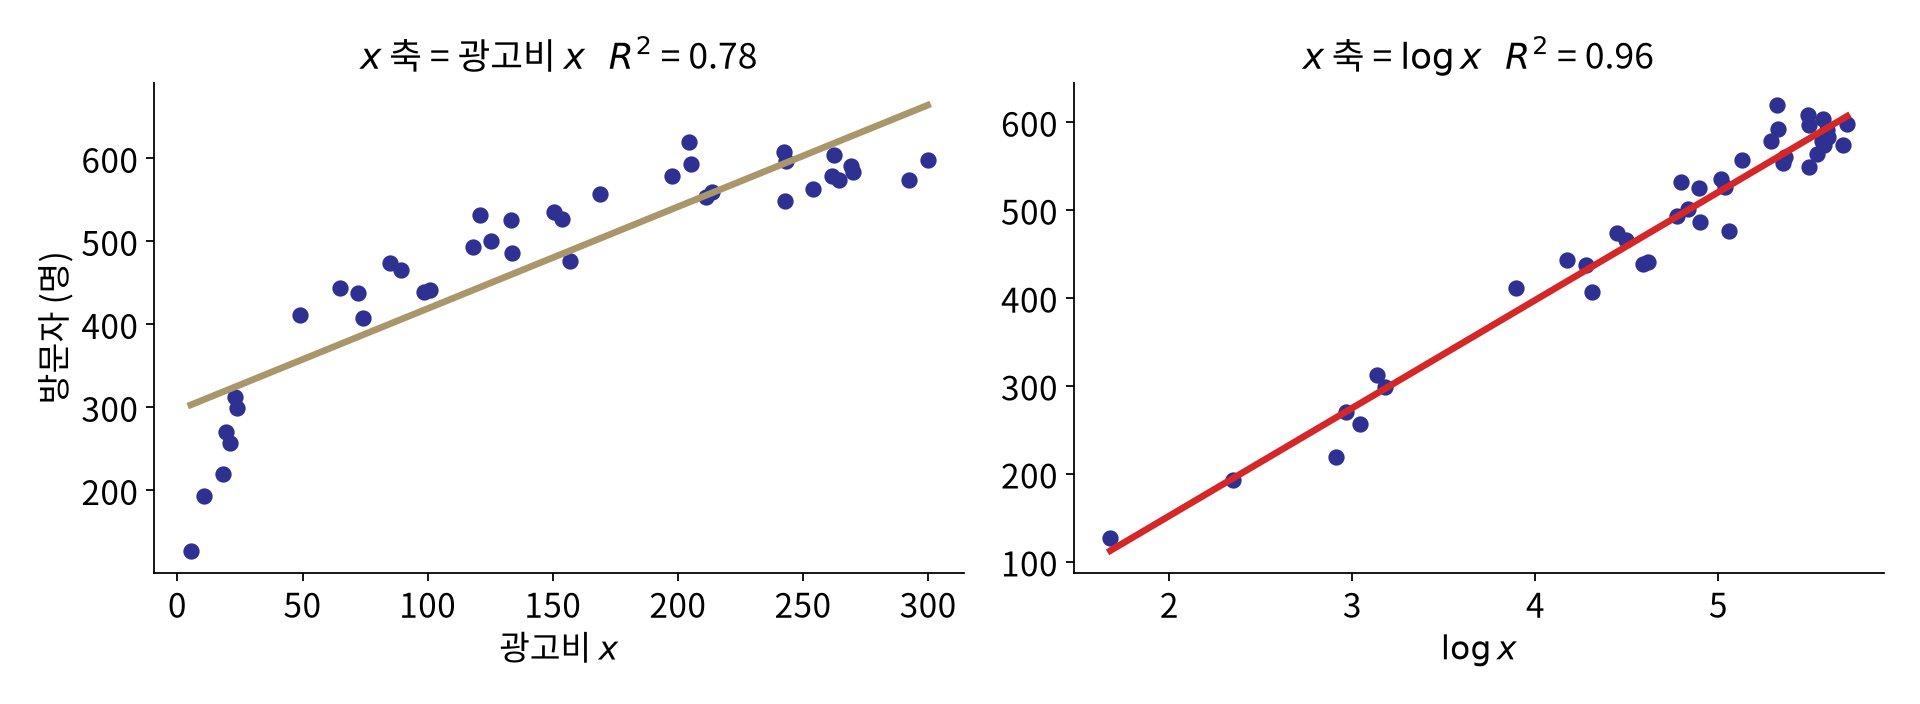
\includegraphics[width=0.9\linewidth]{lr_log.png}\par\vskip0.3em
{\large 광고비 $\to$ 방문자: $x$ 대신 $\log x$ 를 넣으면 \kb{$R^2$ 0.78 $\to$ 0.96}}
\vfill
\note{광고비와 방문자 수입니다. 처음에는 광고비를 늘리면 방문자가 쑥쑥 늘지만, 점점 덜 늘어납니다. 이럴 때는 x 대신 로그 x를 특징으로 넣습니다. 오른쪽처럼 가로축을 로그로 바꾸면 점들이 거의 일직선이 되고, R 제곱이 0.78에서 0.96으로 오릅니다. 이것도 w에 대해서는 선형이니까 선형회귀입니다.}
\end{frame}

% --- 과적합
\begin{frame}{차수를 계속 올리면: 과적합}
\vfill
\centering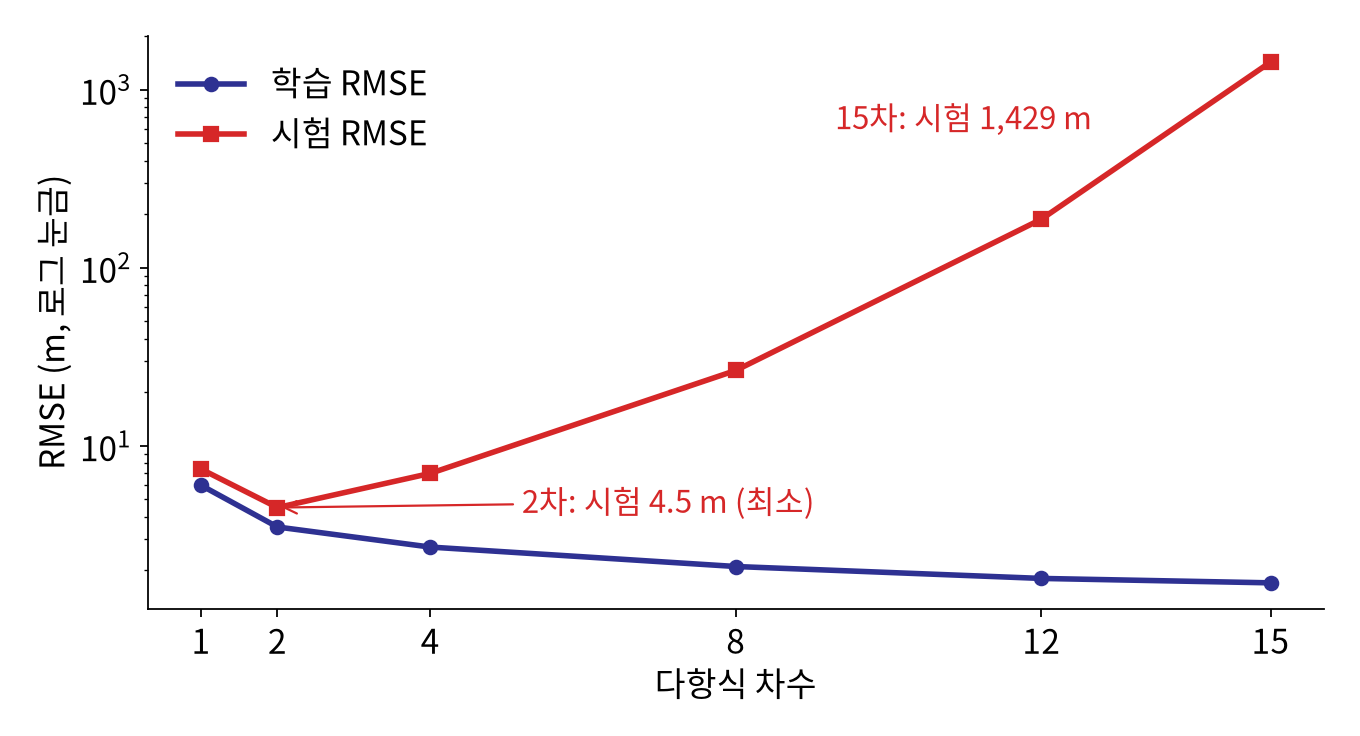
\includegraphics[width=0.62\linewidth]{lr_degree.png}\par\vskip0.3em
{\large 학습 오차는 계속 줄지만, \kq{처음 보는 데이터(시험) 오차는 폭발}한다}
\vfill
\note{그러면 x 세제곱, 네제곱, 계속 넣으면 더 좋아질까요? 제동거리 데이터를 반으로 나눠 반으로 학습하고 나머지 반으로 시험해 봤습니다. 파란 학습 오차는 차수를 올릴수록 계속 줄어듭니다. 그런데 빨간 시험 오차는 2차에서 4.5미터로 가장 작고, 그 뒤로 커져서 15차에서는 1,429미터가 됩니다. 학습 데이터를 외워 버린 겁니다. 이걸 과적합이라고 하고, 5주차 정규화에서 다시 다룹니다.}
\end{frame}

\section{연습}
% --- 문제풀이
\begin{frame}{문제풀이}
\vfill
\begin{enumerate}
\item 데이터 $(1,3), (2,5), (3,7)$, 모델 $h = w_0 + w_1 x$, 지금 $w_0 = 0,\ w_1 = 2$.\\
(a) 세 오차 $h - y$ 는? \; (b) $J$ 는? \; (c) $\partial J/\partial w_0$, $\partial J/\partial w_1$ 는? \; (d) $\alpha = 0.1$ 로 한 걸음 가면?\vskip0.8em
\item 다음 중 선형회귀로 풀 수 있는 모델은? \; (a) $w_0 + w_1 x + w_2 x^3$ \; (b) $w_0 + w_1 \log x$ \; (c) $w_0 + e^{w_1 x}$\vskip0.8em
\item 학습 RMSE 는 계속 줄고 시험 RMSE 는 늘어난다. 무슨 일이 일어나고 있나?
\end{enumerate}
\vfill
\note{1번 답. 예측이 2, 4, 6이니 오차는 모두 마이너스 1입니다. J는 2m분의 1 곱하기 오차 제곱의 합, 6분의 1 곱하기 3, 0.5입니다. w0 기울기는 오차의 평균 마이너스 1, w1 기울기는 오차 곱하기 x의 평균, 마이너스 1, 2, 3의 평균이라 마이너스 2입니다. 한 걸음 가면 w0는 0 빼기 0.1 곱하기 마이너스 1로 0.1, w1은 2 빼기 0.1 곱하기 마이너스 2로 2.2입니다. 2번 답. a와 b는 w에 대해 선형이라 선형회귀, c는 w1이 지수 안에 있어서 아닙니다. 3번 답. 학습 데이터를 외우는 과적합입니다.}
\end{frame}

% --- 실습
\begin{frame}{실습}
\vfill
\centering\begin{tabular}{rl}
\large 1 & 경사하강법 직접 구현: 기울기 두 줄 채우기 $\to$ 7시간 75.3점 재현, 학습률 바꿔 발산 보기\\[0.5em]
\large 2 & 실제 자동차 데이터: 마력 $\to$ 연비, 직선 vs $x^2$ vs $\log x$ 의 $R^2$ 비교\\[0.5em]
\large 3 & 같은 데이터로 차수 올리기: 학습 / 시험 오차로 과적합 찾기
\end{tabular}\vskip1em
Auto MPG (자동차 398대, UCI) \\[0.4em]\href{https://colab.research.google.com/github/SuminHan/book-ml/blob/main/slides/v2/ml1/week02/linear_regression/lab/linear_regression.ipynb}{\textcolor{ksagolddk}{▶ Colab에서 실습 노트북 열기}}
\vfill
\note{실습은 세 부분입니다. 첫째, 오늘 본 기울기 두 줄을 직접 채워서 경사하강법을 구현하고, 7시간 75.3점을 재현합니다. 학습률을 키워서 발산도 직접 봅니다. 둘째, 실제 자동차 398대의 마력과 연비 데이터에서 직선, 제곱 특징, 로그 변환 중 무엇이 가장 잘 맞는지 비교합니다. 셋째, 같은 데이터로 차수를 올려 가며 과적합이 언제 시작되는지 찾습니다.}
\end{frame}

\section{정리}
% --- 정리
\begin{frame}{정리}
\vfill
\centering\large\begin{tabular}{l}
모델 \quad $h = w_0 + w_1 x$ \qquad 비용 \quad 오차 제곱의 평균 $J$\\[0.5em]
경사하강법 \quad 기울기 반대로 한 걸음, 학습률은 적당히\\[0.5em]
곡선도 선형회귀 \quad $x^2$, $\log x$ 를 특징으로 ($w$ 에 대해 선형)\\[0.5em]
차수를 너무 올리면 과적합 \quad 시험 오차로 확인
\end{tabular}
\vfill
\note{정리합니다. 선형회귀는 직선 h를 긋고, 오차 제곱의 평균인 비용 J를 재고, 경사하강법으로 J의 바닥을 찾습니다. 학습률은 적당히 골라야 합니다. 곡선 데이터도 x 제곱이나 로그 x를 특징으로 넣으면 선형회귀로 풀 수 있습니다. 선형은 w에 대해 선형이라는 뜻이니까요. 다만 차수를 너무 올리면 과적합이 생기니, 학습에 쓰지 않은 시험 데이터로 확인해야 합니다.}
\end{frame}
\end{document}
